\documentclass{classeENS}
\usepackage{lipsum}

%----------- Quelques commandes user ----------
\newcommand{\TODO}[1]{\textcolor{red}{TODO: #1}}
%----------------------------------------------

\title{Template rapport ENS } %Titre du fichier

\begin{document}

%----------- Informations du rapport ---------

\titre{Développement et mise à niveau des outils Intranet} %Titre du fichier .pdf
\departement{UFR Sciences et Techniques} 
\matiere{Département d'informatique} 
\motif{Stage -- 2ème année de Master en Informatique Ingénierie Systèmes et Logiciels }

\enseignant{Louis-Claude \textsc{Canon}} %Nom de l'enseignant
\tuteurpcp{Mickaël \textsc{Gros}}
\eleves{Nathan \textsc{Piranda}} %Nom des élèves

%----------- Initialisation -------------------
        
\fairemarges %Afficher les marges
\fairepagedegarde %Créer la page de garde
\addtocontents{toc}{\protect\thispagestyle{empty}}
\tabledematieres %Créer la table de matières
\tabledefigure

%------------ Corps du rapport ----------------

\vspace*{\fill}
\section*{Remerciements}

Tout d'abord, je souhaiterais remercier Monsieur William \textsc{Bosdure}, responsable du service informatique de la Manufacture, qui m'a accordé sa confiance pour que je puisse mener à bien mon stage au sein de son service. \\

Je remercie aussi Monsieur Mickaël \textsc{Gros}, responsables des projets et des stagiaires dans le service informatique. Son suivi, ses conseils et ses réponses à chacune de mes questions ont fait de ce stage une agréable expérience. \\

J'adresse également mes remerciements à Monsieur Louis-Claude \textsc{Canon} pour son suivi et ses consignes pour la rédaction de ce mémoire et à la préparation de la soutenance orale du stage. \\

Je voudrais remercier l'ensemble du département informatique de la Manufacture, notamment le secteur Business Applications \& Projects et Applications Development avec lesquels j'ai partagé leur espace de travail durant ce stage, merci à M. Julien \textsc{Arphant}, M. Maxime \textsc{Berthet}, Mme. Virginie \textsc{Carrez}, M. Frédéric \textsc{Courtet}, M. Claude \textsc{Debost}, M. Madjid \textsc{Nafa}, Mme. Sophie \textsc{Petitalot}, M. Kevin \textsc{Surinon}, M. Tarek \textsc{Tamim} sans oublier l'ensemble du personnel de la Manufacture qui ont fait de ce lieu de travail une agréable expérience. \\

Je voudrais adresser des remerciements spéciaux à Madame Nathalie \textsc{Vallet}, opératrice chez Jaeger-LeCoultre, qui m'a fait découvrir la marque il y a 3 ans et m'a permis d'entrer en contact avec le département informatique pendant les Portes Ouvertes de la Manufacture.
\vspace*{\fill}

\chapter{Introduction}
\section{Contexte du stage}

\section{Missions de stage}

\section{Objectifs du stage}

\chapter{Environnement de stage}
\section{Le Groupe Richemont}
La Compagnie financière Richemont, ou plus simplement Richemont est un groupe spécialisé dans l'industrie du luxe, fondé en 1988 par le milliardaire sud-africain Johann Rupert, actionnaire majoritaire du groupe. \\

Richemont est l’un des leaders mondiaux dans le secteur du luxe, possède vingt Maisons d’envergure internationale dans les secteurs de l'horlogerie (A. Lange \& Söhne, Baume \& Mercier, IWC, Jaeger-LeCoultre, Montblanc, Officine Panerai, Piaget, Vacheron Constantin,...), de la joaillerie (Van Cleef \& Arpels, Cartier, ...), de la mode (Alfred Dunhill, Azzedine Alaïa, Chloé,...) et bien d'autres. \\

Situé à Bellevue, dans le canton de Genève, Richemont a pour objectif le développement de ses marques afin d'assurer la croissance à long terme de son chiffre d'affaires et de son bénéfice tout en veillant à préserver et à promouvoir la réputation et l'intégrité de ses marques.

\section{Jaeger-LeCoultre, manufacture de Haute Horlogerie}
C'est au cœur de la Vallée de Joux, dans le Jura Suisse, que depuis 1833 la Manufacture Jaeger-LeCoultre n'a de cesse de renouveler sa créativité et son inventivité horlogère. Sous un même toit, 180 savoir-faire s'unissent pour insuffler la vie au cœur des montres et animer l'infiniment petit. Dessiner, assembler, décorer ou sertir ; les différentes étapes nécessaires à la création d'un garde-temps Jaeger-LeCoultre sont effectuées par les artisans de la Grande Maison. \\

\begin{figure}[ht]
    \centering
    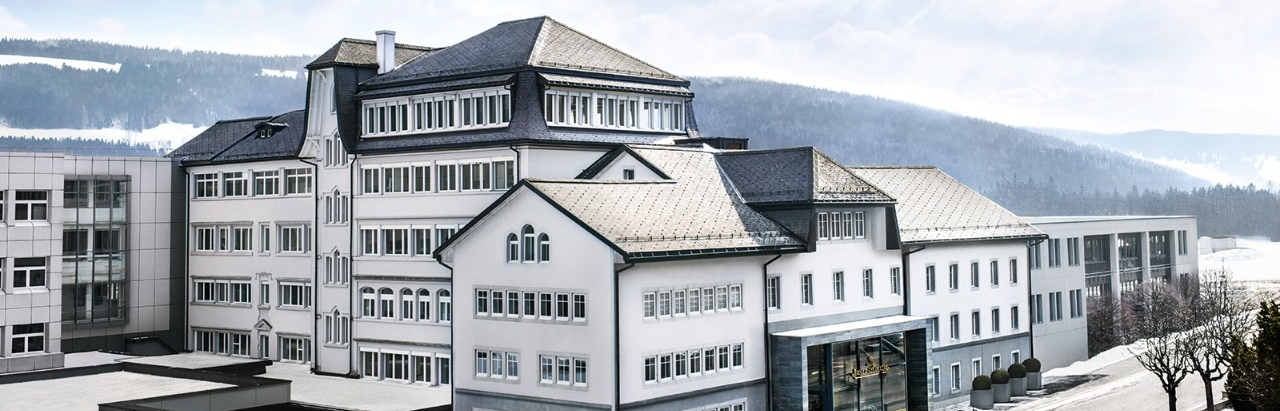
\includegraphics[width=\textwidth]{images/manufacture.jpg}
    \caption{Manufacture Jaeger-LeCoultre}
    \label{fig:manufacture}
\end{figure}

Depuis ses origines, la Maison a conçu et fabriqué plus de 1200 calibres qui lui offrent aujourd'hui une reconnaissance unique dans le monde horloger. Iconiques, ses collections telles que Reverso, née de l'Art déco en 1931, Master, ligne masculine classique et raffinée ou encore Atmos, la pendule au mouvement quasi-perpétuel, font aujourd'hui la fierté de la Manufacture et le bonheur de ses fidèles clients. \\

Première Manufacture horlogère de la Vallée de Joux, elle compte environ 1200 collaborateurs réunis sur une surface de 25000 m$^{2}$. Parmi eux, 1000 sont dédiés à l’activité industrielle dont environ 200 horlogers. \\

Jaeger-LeCoultre s'illustre aussi dans la fabrication des complications des montres. On parle de complication quand une montre donne d'autres informations que l'heure. On trouve des montres labellisées "Grande Complication" avec des composants affichant des répétitions minute, des calendriers perpétuels, des chronomètres, etc... \\

Parmi les créations qui ont marqué l'histoire de la Manufacture, on trouve la pendule Atmos dont les mécanismes se remontent avec les changements de la température ambiante. La création du calibre 101 qui détient encore aujourd'hui le record du plus petit calibre mécanique au monde depuis 1929. On trouve aussi leur collection phare : la Reverso, qui possède un cadran reversible pour protéger la montre. Elle était pensée au début pour les matchs de polo. \\
On trouve aussi dans les gammes de produits de la marque (voir Figure~\ref{fig:products}), de gauche à droite : Master Extreme, Hybris Artistica, Master, Hybris Mechanica, Reverso, Rendez-vous, Polaris, Duomètre, Geophysics et Atmos.

\begin{figure}[ht]
    \centering
    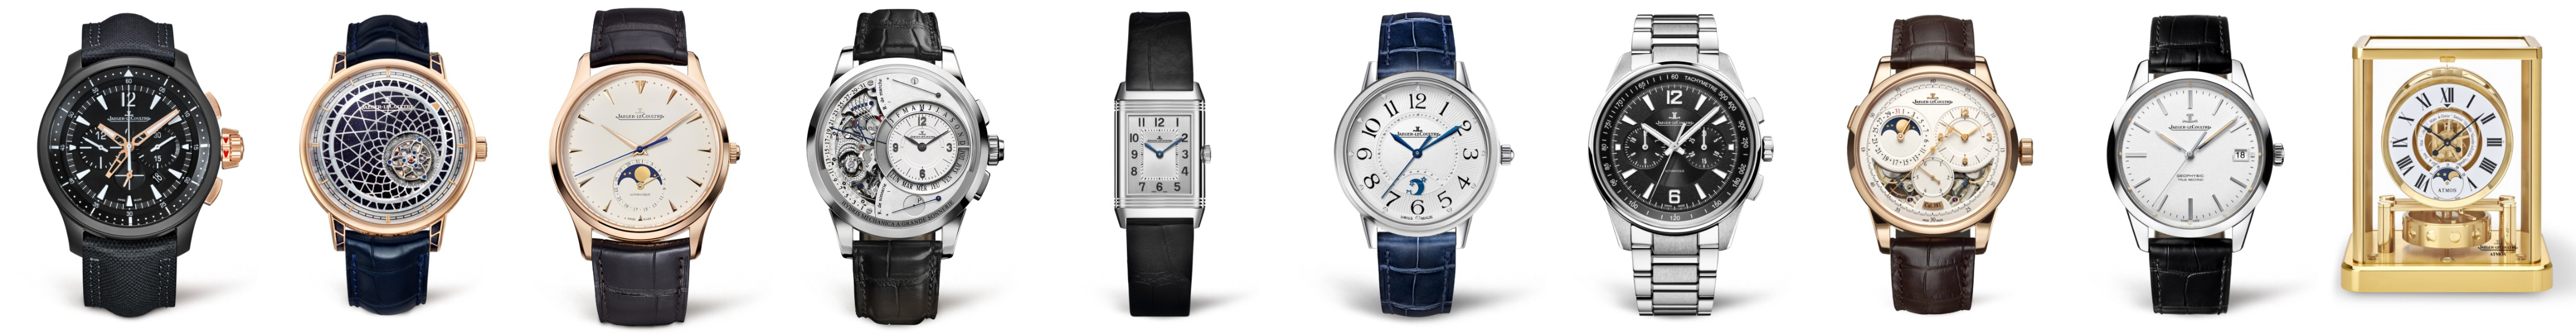
\includegraphics[width=\textwidth]{images/all_products.png}
    \caption{Les différentes gammes de produits Jaeger-LeCoultre.}
    \label{fig:products}
\end{figure}

La marque possède un réseau de boutiques composé de 53 Boutiques Internes et 80 Boutiques Externes à travers le monde. Ces boutiques représentent la clé du développement international de notre Marque. Vous trouverez en Figure~\ref{fig:boutiques} une carte avec la vision d'ensemble de nos boutiques dans le monde.

\begin{figure}[ht]
    \centering
    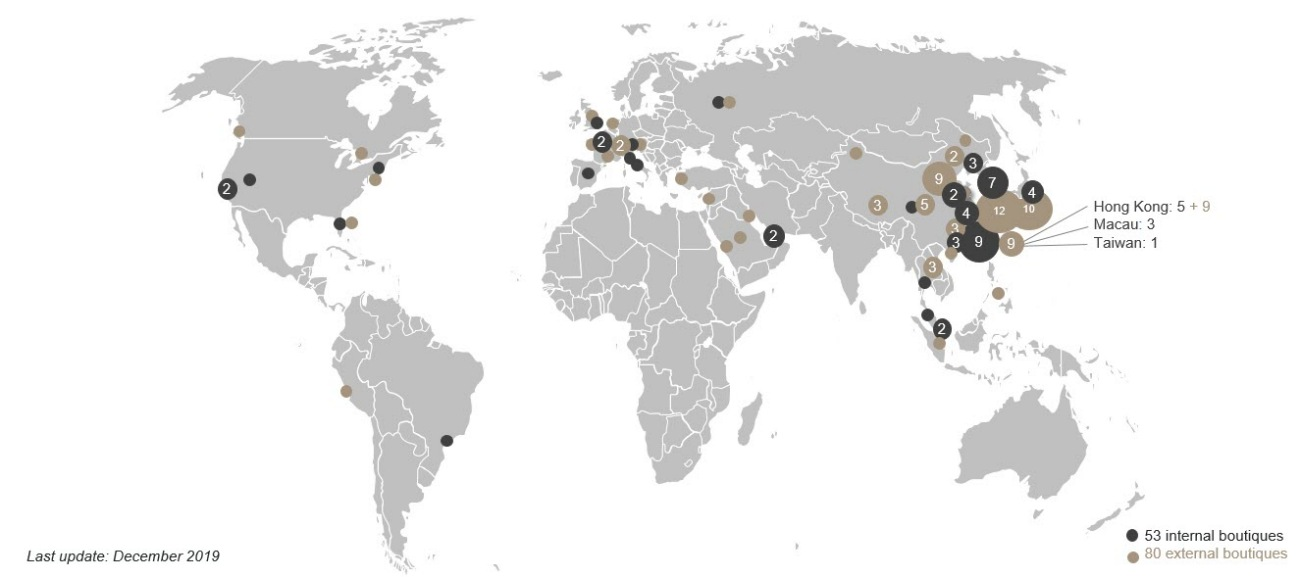
\includegraphics[width=\textwidth]{images/boutiques.jpg}
    \caption{Les boutiques Jaeger-LeCoultre dans le monde.}
    \label{fig:boutiques}
\end{figure}



\section{Le service \textit{Information system \& Organization}}
Le département Système d’Information et Organisation modernise et déploie le système d’information de l’entreprise : amélioration de sa productivité, gestion des changements d’organisation liés à la mise en place de nouveaux systèmes et optimisation et sécurisation de l’infrastructure. \\

Le département a pour missions principales : \\
\begin{itemize}
    \item Définir les orientations du système d’information afin de répondre aux demandes et à la stratégie générale de l’entreprise. Le département est en charge des problématiques d’organisation, en tant qu’aide à la décision et à la conception de solutions.
    \item Suivre la mise en œuvre des projets informatiques de l’entreprise. Il maîtrise les risques financiers, organisationnels et techniques, et veille au respect des délais. Attentif à la bonne adéquation entre les équipes et les moyens mis à disposition, il effectue les choix d’internalisation ou d’externalisation des activités.
    \item Le département est en charge de l’animation des projets et les relations avec les services concernés. Il fait la passerelle entre les équipes internes, les fournisseurs informatique et les équipes Richemont informatique, sécurité et digitale.\\
\end{itemize}

\begin{figure}[ht]
    \centering
    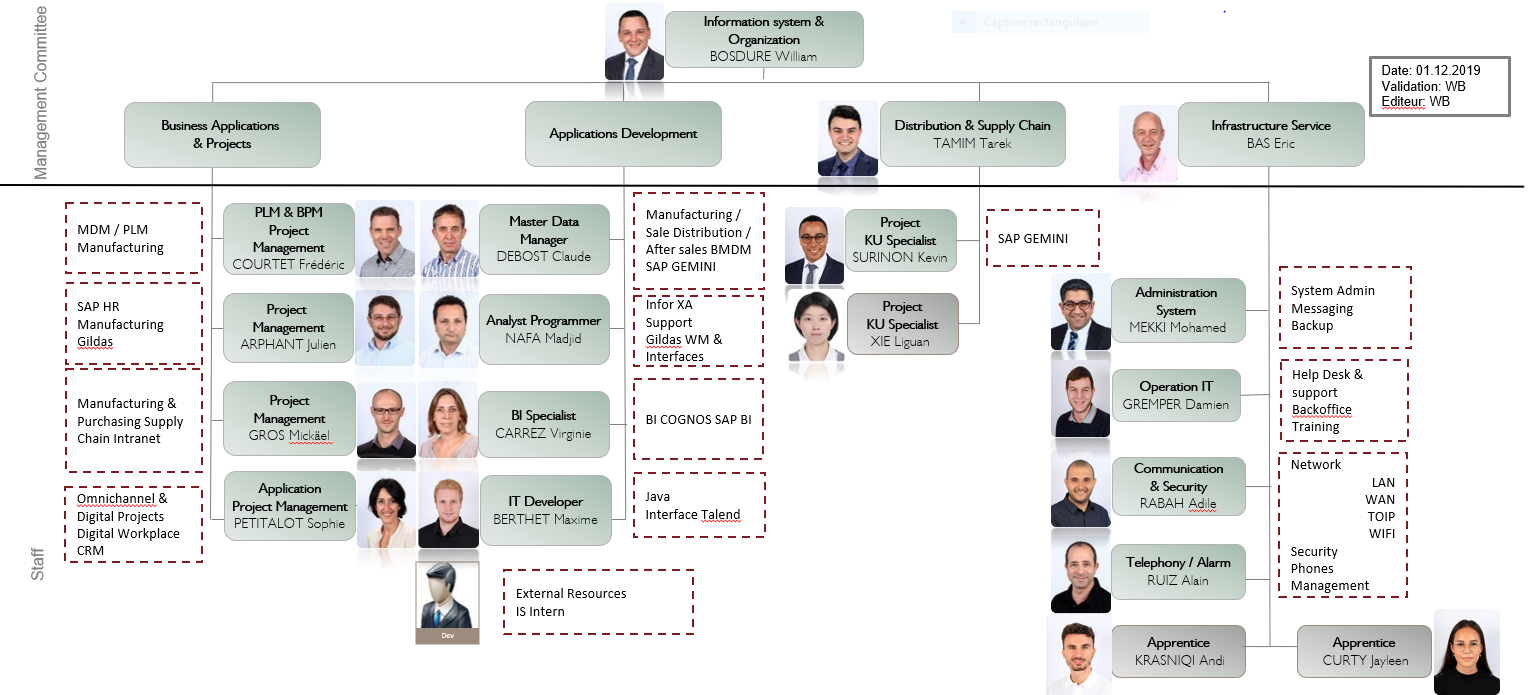
\includegraphics[width=\textwidth]{images/organisation.PNG}
    \caption{Organisation du service informatique.}
    \label{fig:organisation}
\end{figure}

Le graphique en figure~\ref{fig:organisation} montre l'organisation du département, on compte trois pôles de compétences qui regroupent de nombreux métiers :

\paragraph{Infrastructure \& Nouvelles technologies}L’équipe assure la mise en place, la maintenance du parc de matériel et des logiciels sur les sites du Sentier et de Porrentruy, plus de 1200 équipements répartis entre des PCs, écrans tactiles, serveurs, TV, imprimantes, téléphones. Ce pôle est aussi en charge de la sécurité des systèmes.

\paragraph{SAP Distribution \& Supply Chain}L’équipe assure le déploiement de nos ressources et processus sur les plateformes logistiques et Supply Chain du Groupe Richemont pour garantir un flux efficace entre la sortie des produits de la Manufacture vers le client final.

\paragraph{Projets \& Développements d’applications}Chefs de Projets et développeurs accompagnent tous les secteurs de l’entreprise dans la conduite de leurs projets les plus complexes : de la conception produit (PLM) à la gestion du client final (Dpt Retail, CRM-Digital) en passant par la Production (gestion de notre ERP) et la Supply Chain (optimisation des flux d’approvisionnement et de livraison).

\chapter{Organisation et méthodes de travail}
\section{Une organisation inspirée des méthodes Agiles}
\section{Outils organisationnels}
\section{Outils de développement}

\chapter{Mise à niveau des outils Intranet}
\section{Rappel du contexte}
\section{Analyse du besoin}
\section{Migration des applications}
\section{Résultats obtenus}

\chapter{Automatisation des tests}
\section{Analyse du besoin}
\section{Présentation de Selenium}
\section{Quelques exemples}
\section{Résultats obtenus}

\chapter{Activités annexes}
\section{PortailManufacture}
\section{eCardCreator}

\chapter{Conclusion}
\input{report/conclusion}

\bibliographystyle{plain}
\bibliography{sources.bib}

\end{document}